\documentclass[10pt,twoside,slovak,a4paper]{article}
\usepackage[slovak]{babel}
%\usepackage[T1]{fontenc}
\usepackage[IL2]{fontenc}
\usepackage[utf8]{inputenc}
\usepackage{graphicx}
\usepackage{url} % príkaz \url na formátovanie URL
\usepackage{hyperref}
\usepackage{graphicx}
\graphicspath{ {./images/} }
\usepackage{cite}

\pagestyle{headings}


\title{Rozpoznávanie objektov v reálnom čase pre autonómne vozidlá\thanks{Semestrálny projekt v predmete Metódy inžinierskej práce, ak. rok 2021/22}}
\author{Vladimír Kočík\\[2pt]
	{\small Slovenská technická univerzita v Bratislave}\\
	{\small Fakulta informatiky a informačných technológií}\\
	{\small \texttt{xkocik@stuba.sk}}
	}

\date{November 2021}



\begin{document}
\maketitle
\begin{abstract}

Vývoj autonómnych vozidiel neustále pokračuje, a každým dňom sa stávajú metódy využívané samoriadiacimi autami rýchlejšie a zároveň bezpečnejšie. Aj keď dnes je o komerčnom využití týchto vozidiel ešte priskoro uvažovať, myslím že o niekoľko rokov sa to zmení. Jedna z motivácií je znížiť počet dopravných nehôd, keďže dnes je väčšina z nich spôsobená práve chybou alebo nepozornosťou vodiča. V mojom článku som sa chcel zamerať na metódy využívané autonómnymi vozidlami na rozpoznávanie hranice cesty a objektov na ceste a ako môže vyzerať plánovanie bezpečného zaraďovania auta vo dvojprúdových a trojprúdových cestách.

%Keďže najnovší výskum nie je pravidelne publikovaný a sprístupnený verejnosti, je mnou opísané metódy sú dnes nahradené lepšími a efektivnejšími, no stále majú hodnotu pri študovaní vývoja týchto technológií. Samozrejme to nie je niečo, z čoho by sa každý dokázal odborník po prečítaní pár článkov, aj moje porozumenie témam je limitované, no mojou snahou bude čo najbližšie vysvetliť danú tému.

\end{abstract}

\section{Úvod} 

Pri autonómnych vozidlách je kľúčové presné zaznamenanie prostredia, lokalizácia, mapovanie a iné technológie ktoré čerpajú dáta z kamery, taktiež GPS, IMU(Inertial Measurement Unit), odometria kolies, senzory LIDAR(Light Detection and Ranging) 


\cite{6629552}

\section{Rozpoznávanie čiar na ceste}

Prvé algoritmy vychádzajúce z algoritmu videnia boli veľmi nepresné, a preto boli často spájané s inými algoritmami, ktoré filtrovali farby, hrany, pracovali s perspektívou a metódami ako Sobel, sliding widows search (SWS), the least-squares methond(LMS) a bird-eye view(BEV). Pomocou týchto filtrov dokázal algoritmus rozpoznať rovné čiary na ceste, no po niekoľkých testovaniach sa zistilo že je to stále veľmi nepresné, pretože sa na ceste môže nachádzať veľa rušivých faktorov, či sú to objekty na ceste, vozidlá, svetlosť, stav vozovky alebo aj zlé počasie. 
Preto veľmi dôležitou časťou rozpoznávania čiar je použitie algoritmov pre supervised and unsupervised learning. Použitím neurálnych sietí -convolutional neural networks (CNNs), a známy CNN model, AlexNet bol navrhnutý a je okolo neho postavených mnoho algoritmov. Neustálym zberom dát a obrovským množstvom iterácií sa presnosť stále zvyšuje.

Metóda pre rozpoznávanie čiar na základe unsupervised learning algoritmu je odstrániť z obrazu všetky nedôležité údaje, tak aby ostaly len hlavné hrany. Na to je v tomto prípade použitý algoritmus Canny. Ďalej, aby sa predišlo falošnému pozitívu, sú pomocou ROI (Regions of Interest) filtrované tie objekty, v ktorých sa nepredpokladá že sa v nich nachádzajú čiary ale práve iné objekty na základe ich pozície na obrazovke. Pre lepšie zobrazenie používame funkciu OpenCV aby sme sa dostali do BEV, teda vtáčiej perspektívy. Po transformácií sa použije SWS aby sa našiel rozdiel medzi pravou a ľavou čiarou. 

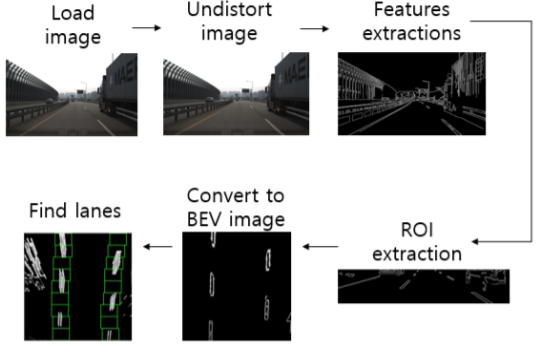
\includegraphics{find_lanes2}





\cite {KSII}
\cite {9179748}
\cite{tiis:22283}
\cite{tiis:23914}


\section{Rozpoznávanie objektov}


\cite {9337402}
\cite {9253253}

\section{Plánovanie - bezpečné zaraďovanie}


\cite {9034121}

\section{Záver}

\bibliography{zdroje}
\bibliographystyle{plain}

\end{document}